\section{Gridalt - Alternate Grid Package}
\label{sec:pkg:gridalt}
\begin{rawhtml}
<!-- CMIREDIR:package_gridalt: -->
\end{rawhtml}

\subsection {Introduction} 
To take advantage of a `high end' turbulence parameterization
(and convection parameterization), the vertical resolution near the surface
must be increased substantially as compared to the vertical resolution needed
aloft. This cannot be accomplished if the high end physics is computed using 
the $p^*$ coordinate currently in use in the MIT gcm. 

The gridalt package was developed to allow the high end atmospheric physics 
(fizhi) physics to be run on a separate grid from the hydrodynamics. The package
could (with some user modification) be used in conjunction with other packages 
or for other calculations within the GCM. For the case of the atmospheric 
physics, a modified $p^*$ coordinate, which adds additional levels between
the lower levels of the existing $p^*$ grid (and perhaps between the levels near 
the tropopause as well), is implemented. The vertical discretization is
different for each grid point, although it consist of the same number of 
levels. This is illustrated as follows:
\begin{figure}[htbp]
\vspace*{-0.4in}
\begin{center}
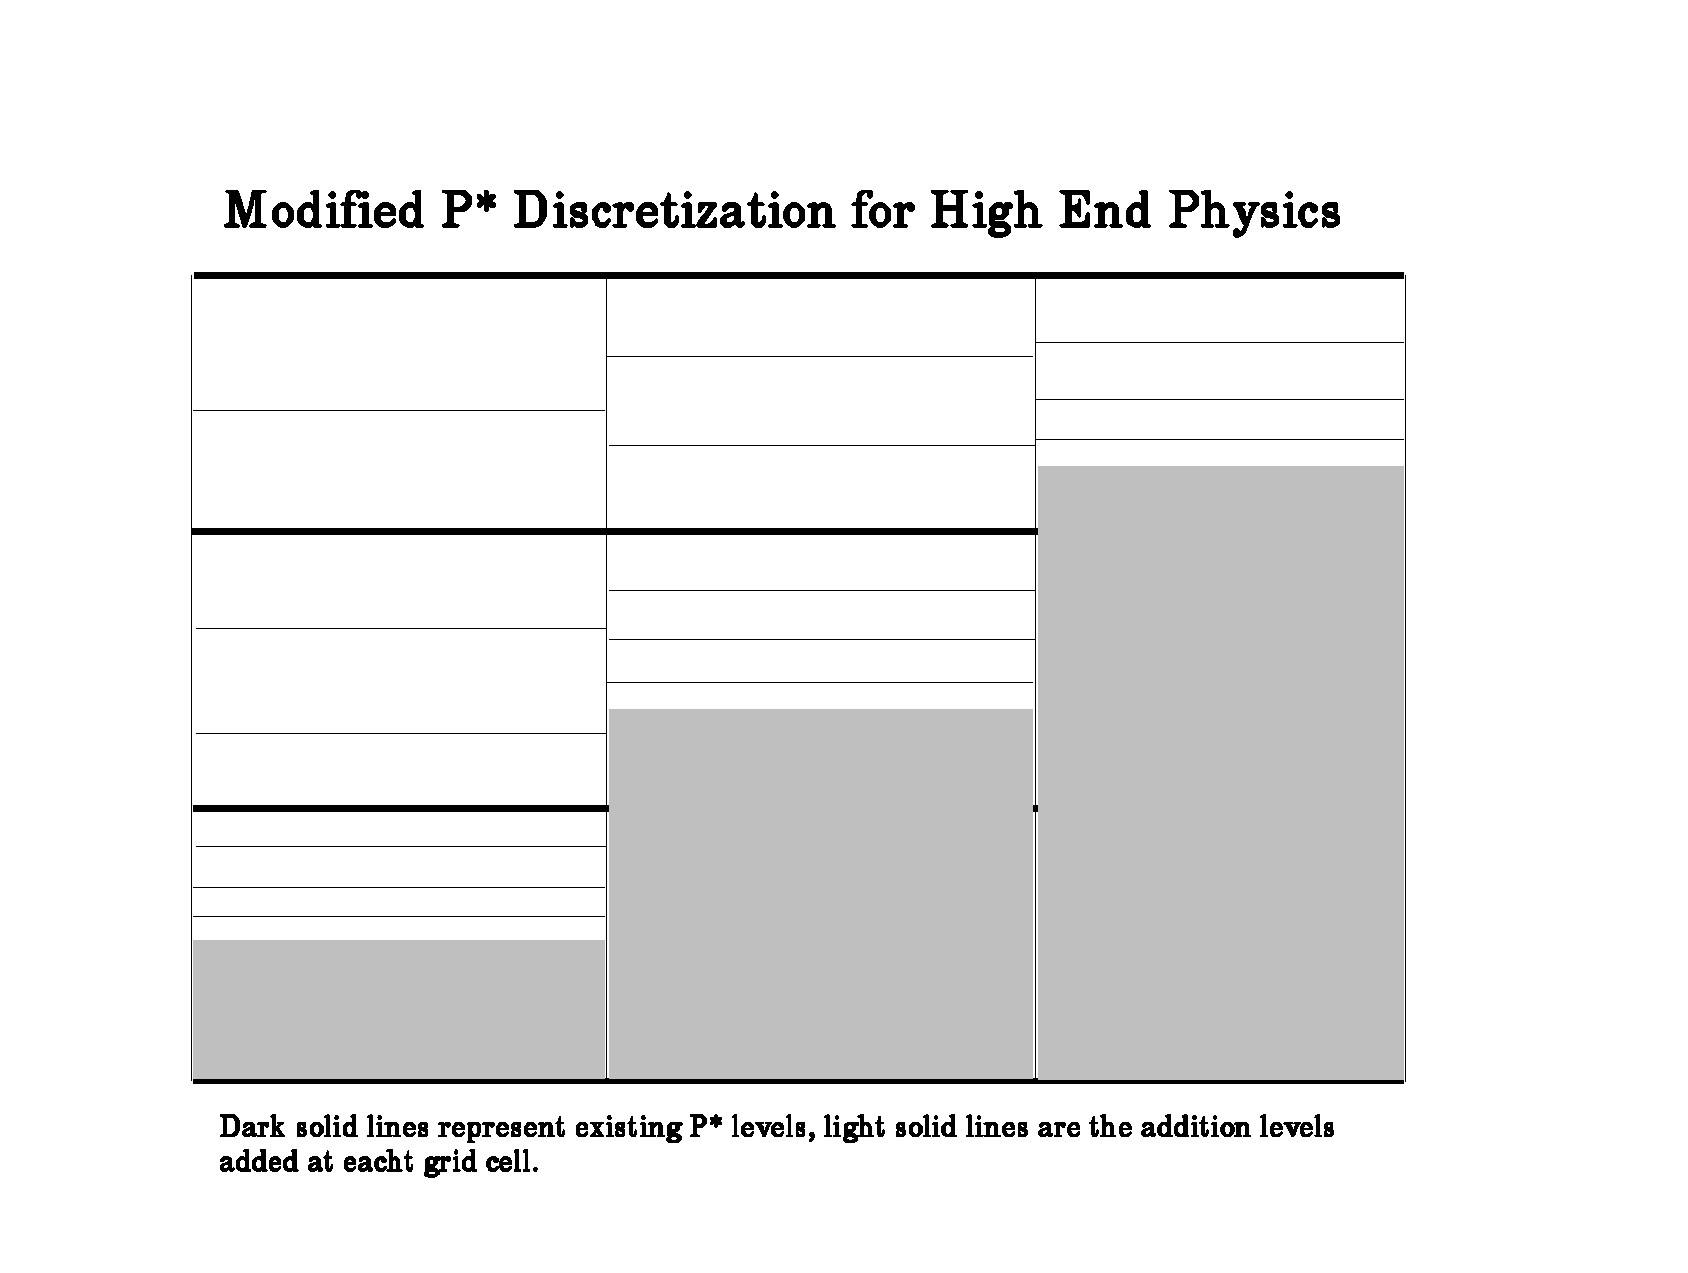
\includegraphics[height=2.4in]{vertical.eps}
\end{center}
\end{figure}

\vspace*{-0.5in}
In addition to computing the physical forcing terms of the momentum,
thermodynamic and humidity equations on the modified (higher resolution)
grid, the higher resolution structure of the atmosphere (the boundary
layer) is retained between calculations. This neccessitates a second 
set of evolution equations for the atmospheric state variables on the 
modified grid. If the equations for the evolution of the state
on $p^*$ can be expressed as:
\[
\left . {\partial U \over {\partial t}} \right |_{p^*}^{total} = 
\left . {\partial U \over {\partial t}} \right |_{p^*}^{dynamics} + 
\left . {\partial U \over {\partial t}} \right |_{p^*}^{physics}
\]
where the physics forcing terms on $p^*$ have been computed from a
mapping from the modified grid, then an additional set of equations
to govern the evolution of $U$ on the modified grid are written:
\[
\left . {\partial U \over {\partial t}} \right |_{p^{*m}}^{total} = 
\left . {\partial U \over {\partial t}} \right |_{p^{*m}}^{dynamics} + 
\left . {\partial U \over {\partial t}} \right |_{p^{*m}}^{physics} +
\gamma ({\left . U \right |_{p^*}} - {\left . U \right |_{p^{*m}}})
\]
where $p^{*m}$ refers to the modified higher resolution grid, and
the dynamics forcing terms have been mapped from the $p^*$ space.
The last term on the RHS is a relaxation term, meant to constrain
the state variables on the modified vertical grid to `track' the
state variables on the $p^*$ grid on some time scale, $\gamma$.

\subsection {Key subroutines, parameters and files } 

\subsection {Dos and donts}

In the context of a Held-Suarez type of model experiment (located
in the fizhi-hs.cs-32x32x10 verification experiment) with
topography, the forcing terms which represent the physics are computed on 
the modified grid. The forcing terms are computed as functions of the
state variables on the modified grid. The tendencies are then interpolated
to the standard grid

\subsection {Gridalt Reference} 
